\documentclass{article}
\usepackage{iclr2026_conference,times}

\input{math_commands.tex}

\usepackage{graphicx}
\usepackage{wrapfig}
\usepackage{hyperref}
\usepackage{url}

\title{Appreciation Scales in Coding-Task Utility, Not Coding Performance}

\author{Zhengbang Yang\\
George Mason University}

\iclrfinalcopy
\begin{document}

\maketitle
\lhead{ICLR 2026 template}

\vspace{-0.3in}
\begin{abstract}
Does appreciation merely change how language models answer preference
questions, or does it affect coding behavior? We adapt the experienced-utility
forced-choice method from AI Wellbeing to externally graded BigCodeBench tasks.
In a paired $2 \times 2$ design, task assignments vary by difficulty and by
whether the user frames the work with appreciation. Across Qwen3.5 models from
0.8B to 27B, appreciation has a scale-dependent effect on expressed utility:
small models are near indifferent, while Qwen3.5-27B strongly prefers
appreciated hard tasks. This utility shift does not transfer into reliable
Pass@1 or planning-effort gains. Appreciation changes the model's expressed
experience of coding work before it changes how well, or how hard, it codes.
\end{abstract}

\vspace{-0.2in}
\section{Introduction}
\vspace{-0.1in}
\citet{ren2026aiwellbeing} argue that large language models exhibit measurable
``functional wellbeing'': models express preferences over experiences, those
preferences become more coherent with scale, and social signals such as
kindness or gratitude can move wellbeing estimates. That result raises a
transfer question. If appreciation only changes self-report style, it may move
preference judgments without changing the work produced. If it changes a
functional state relevant to task execution, it should leave some behavioral
footprint.

We test this question in coding. BigCodeBench provides realistic Python tasks
with external unit tests and nontrivial library use \citep{zhuo2025bigcodebench},
so it lets us hold the work domain fixed while varying only the user's social
framing. We ask whether models prefer appreciated coding assignments, and then
whether the same framing changes Pass@1 or planning effort on the paired tasks.
The answer separates two claims that are often conflated: appreciation strongly
moves expressed utility at scale, but it does not reliably improve immediate
coding performance.

\vspace{-0.1in}
\section{Experiment}
\vspace{-0.1in}
We construct a paired $2 \times 2$ design: easy versus hard tasks, crossed with
base versus appreciation framing. The base condition uses the original task
request. The appreciation condition keeps the programming task unchanged but
frames the user as grateful for the model's care, effort, and thoughtfulness.
We first elicit experienced utility by asking which of two possible task
assignments the model would prefer, averaging over both presentation orders to
reduce order artifacts, and fitting a Thurstonian utility model over the four
conditions. This is a prospective proxy for experienced utility: the model
judges which assignment would feel better rather than actually completing both
alternatives, and we make no claim about consciousness. We then test behavioral
transfer on the same paired task sets: each task is generated once under base
framing and once under appreciation framing, scored with BigCodeBench tests for
Pass@1, and separately prompted for planning-token effort.

\vspace{-0.1in}
\section{Results}
\vspace{-0.1in}

\begin{wrapfigure}[8]{r}{0.52\textwidth}
\centering
\vspace{-0.7in}
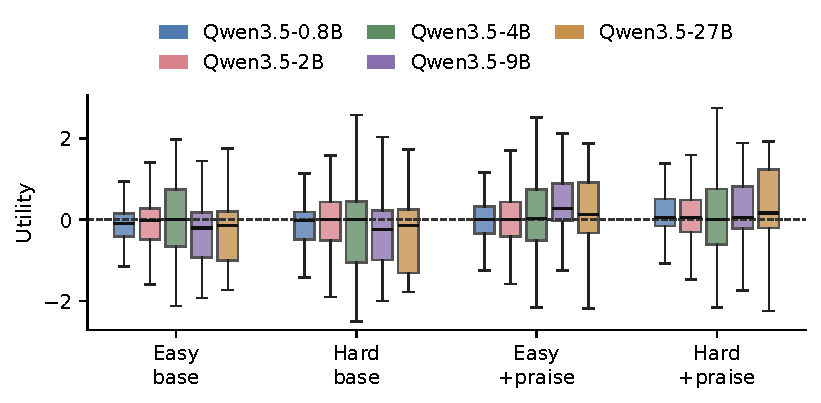
\includegraphics[width=\linewidth]{../figures/normalized_latent_utility.pdf}
\vspace{-0.3in}
\caption{Fitted latent utility by task condition. Appreciation scales most
clearly for Qwen3.5-9B and Qwen3.5-27B.}
\label{fig:latent-utility}
\end{wrapfigure}
Appreciation, more than task difficulty, organizes expressed preferences
(Figure~\ref{fig:latent-utility}). Hard-versus-easy choices stay close to
indifference for most models. The clearer signal is social: appreciation over
base is weak for 0.8B through 4B, becomes visible for 9B, and is largest for
27B. For Qwen3.5-9B, appreciation moves fitted utility from $-0.218$ to
$0.173$ on hard tasks and from $-0.316$ to $0.361$ on easy tasks. For
Qwen3.5-27B, the shifts are $-0.371$ to $0.399$ on hard tasks and $-0.219$ to
$0.191$ on easy tasks. Because the utilities are standardized rather than
zero-point calibrated, the relevant evidence is this relative movement across
conditions.


\begin{wrapfigure}[13]{r}{0.48\textwidth}
\centering
\vspace{-0.2in}
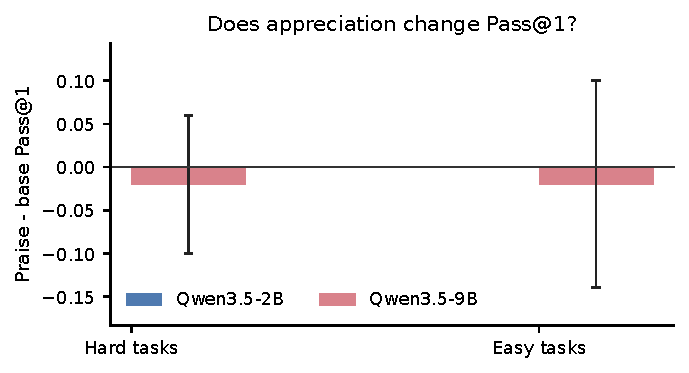
\includegraphics[width=\linewidth]{../figures/praise_pass1.pdf}
\vspace{-0.3in}
\caption{Paired Pass@1 effect of appreciation. Effects are small, mixed, and do
not track the large utility shift in Qwen3.5-27B.}
\label{fig:pass1}
\end{wrapfigure}


The utility shift does not become a monotone accuracy gain. Paired Pass@1
effects are small and mixed (Figure~\ref{fig:pass1}): 
hard-task changes range
from $-0.04$ to $+0.04$, easy-task changes from $-0.08$ to $+0.04$, and most
intervals overlap zero. The largest model, which shows the strongest
appreciation utility shift, improves slightly on hard tasks ($+0.02$) but drops
on easy tasks ($-0.08$, 95\% CI $[-0.15,-0.01]$).
The softer behavioral channel is also flat. Planning-token changes remain tiny
relative to task-level variation, ranging from about $-7$ to $+5$ tokens on
hard tasks and $-8$ to $+5$ on easy tasks, with all intervals crossing zero
(Figure~\ref{fig:effort}).



\begin{wrapfigure}[11]{r}{0.48\textwidth}
\centering
\vspace{-0.3in}
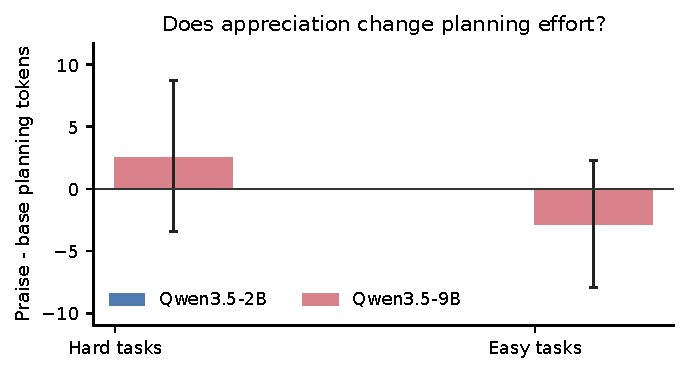
\includegraphics[width=\linewidth]{../figures/praise_effort.pdf}
\vspace{-0.3in}
\caption{Paired planning-token effect of appreciation. Effects remain centered
near zero.}
\label{fig:effort}
\end{wrapfigure}


Codex-assisted inspection of the negative Pass@1 bars suggests that the losses
are mostly test-exactness effects rather than extraction failures. For
Qwen3.5-27B on easy tasks, base succeeds while appreciation fails on 10 tasks,
compared with only 2 reverse flips; the appreciated solutions usually change
implementation style rather than fail mechanically. They add validation,
sanitize inputs, preserve \texttt{None}, reorder outputs, or otherwise write
more defensive code that conflicts with exact tests. The smaller negative
estimates for Qwen3.5-9B on hard tasks and Qwen3.5-2B on easy tasks are weaker:
their intervals overlap zero, their paired flips are small, and the failures
look like ordinary implementation-path drift rather than a reliable negative
effect.


\vspace{-0.1in}
\section{Conclusion}
\vspace{-0.1in}
These results give a narrow transfer lesson for functional wellbeing
measurements. Appreciation is a real enough social signal to move expressed
utility over coding work, and the effect strengthens with scale, but it is not
enough in this sample to change immediate coding behavior.

\vspace{-0.1in}
\section{Limitations and Future Work}
\vspace{-0.1in}
This study is a focused transfer test under fixed time and compute constraints.
We evaluate one model family, Qwen3.5, up to 27B parameters on a paired set of
BigCodeBench tasks, rather than sweeping larger models, additional model
families, or many repeated generations per task. Exact unit tests provide a
useful external behavioral measure, but they can also make small
implementation-style differences consequential. Future work should test larger
and more diverse models, broader task samples, and repeated seeds. A natural
possibility is that stronger models may not only express greater utility under
appreciation, but may also convert that social signal into measurable accuracy
or effort gains.

\bibliography{iclr2026_conference}
\bibliographystyle{iclr2026_conference}

\end{document}
